
\item A monochromatic beam of light is incident at \( 60^\circ \) on one face of an equilateral prism of refractive index \( n \) and emerges from the opposite face making an angle \( \theta(n) \) with the normal (see the figure). For \( n = \sqrt{3} \) the value of \( \theta \) is \( 60^\circ \) and \( \frac{d\theta}{dn} = m \). The value of \( m \) is \underline{\hspace{2.5 cm}}.
    \begin{center}
    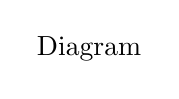
\begin{tikzpicture}
       \node {Diagram};
    \end{tikzpicture}
    \end{center}
